\documentclass{article}

% Packages required by doxygen
\usepackage{calc}
\usepackage{doxygen}
\usepackage{graphicx}
\usepackage[utf8]{inputenc}
\usepackage{makeidx}
\usepackage{multicol}
\usepackage{multirow}
\usepackage{textcomp}
\usepackage[table]{xcolor}

% NLS support packages
\usepackage{polski}
\usepackage[T1]{fontenc}

% Font selection
\usepackage[T1]{fontenc}
\usepackage{mathptmx}
\usepackage[scaled=.90]{helvet}
\usepackage{courier}
\usepackage{amssymb}
\usepackage{sectsty}
\renewcommand{\familydefault}{\sfdefault}
\allsectionsfont{%
  \fontseries{bc}\selectfont%
  \color{darkgray}%
}
\renewcommand{\DoxyLabelFont}{%
  \fontseries{bc}\selectfont%
  \color{darkgray}%
}

% Page & text layout
\usepackage{geometry}
\geometry{%
  a4paper,%
  top=2.5cm,%
  bottom=2.5cm,%
  left=2.5cm,%
  right=2.5cm%
}
\tolerance=750
\hfuzz=15pt
\hbadness=750
\setlength{\emergencystretch}{15pt}
\setlength{\parindent}{0cm}
\setlength{\parskip}{0.2cm}
\makeatletter
\renewcommand{\paragraph}{%
  \@startsection{paragraph}{4}{0ex}{-1.0ex}{1.0ex}{%
    \normalfont\normalsize\bfseries\SS@parafont%
  }%
}
\renewcommand{\subparagraph}{%
  \@startsection{subparagraph}{5}{0ex}{-1.0ex}{1.0ex}{%
    \normalfont\normalsize\bfseries\SS@subparafont%
  }%
}
\makeatother

% Headers & footers
\usepackage{fancyhdr}
\pagestyle{fancyplain}
\fancyhead[LE]{\fancyplain{}{\bfseries\thepage}}
\fancyhead[CE]{\fancyplain{}{}}
\fancyhead[RE]{\fancyplain{}{\bfseries\leftmark}}
\fancyhead[LO]{\fancyplain{}{\bfseries\rightmark}}
\fancyhead[CO]{\fancyplain{}{}}
\fancyhead[RO]{\fancyplain{}{\bfseries\thepage}}
\fancyfoot[LE]{\fancyplain{}{}}
\fancyfoot[CE]{\fancyplain{}{}}
\fancyfoot[RE]{\fancyplain{}{\bfseries\scriptsize Wygenerowano Cz, 19 mar 2015 01\-:08\-:41 dla Lab02 -\/ podstawowe struktury danych programem Doxygen }}
\fancyfoot[LO]{\fancyplain{}{\bfseries\scriptsize Wygenerowano Cz, 19 mar 2015 01\-:08\-:41 dla Lab02 -\/ podstawowe struktury danych programem Doxygen }}
\fancyfoot[CO]{\fancyplain{}{}}
\fancyfoot[RO]{\fancyplain{}{}}
\renewcommand{\footrulewidth}{0.4pt}
\renewcommand{\chaptermark}[1]{%
  \markboth{#1}{}%
}
\renewcommand{\sectionmark}[1]{%
  \markright{\thesection\ #1}%
}

% Indices & bibliography
\usepackage{natbib}
\usepackage[titles]{tocloft}
\setcounter{tocdepth}{3}
\setcounter{secnumdepth}{5}
\makeindex

% Hyperlinks (required, but should be loaded last)
\usepackage{ifpdf}
\ifpdf
  \usepackage[pdftex,pagebackref=true]{hyperref}
\else
  \usepackage[ps2pdf,pagebackref=true]{hyperref}
\fi
\hypersetup{%
  colorlinks=true,%
  linkcolor=blue,%
  citecolor=blue,%
  unicode%
}

% Custom commands
\newcommand{\clearemptydoublepage}{%
  \newpage{\pagestyle{empty}\cleardoublepage}%
}


%===== C O N T E N T S =====

\begin{document}

% Titlepage & ToC
\hypersetup{pageanchor=false}
\pagenumbering{roman}
\begin{titlepage}
\vspace*{7cm}
\begin{center}%
{\Large Lab02 -\/ podstawowe struktury danych }\\
\vspace*{1cm}
{\large Mateusz Krawczuk, nr indeksu 209147}\\
\vspace{0.5cm}
{\large Wygenerowano przez Doxygen 1.8.6}\\
\vspace*{0.5cm}
{\small Cz, 19 mar 2015 01:08:41}\\
\end{center}
\end{titlepage}
\pagenumbering{arabic}

%--- Begin generated contents ---
\part{Streszczenie}
Niniejszy dokument zawiera wyniki pomiaru czasu, którego potrzebował mój komputer na wykonanie operacji mnożenia przez 2 na zestawach danych o długościach od 1 do 10e8 elementów. Zawiera także dokumentację kodu programu użytego do wykonania tego badania.

\part{Sprawozdanie}
Obliczenia wykonano na 64-bitowym procesorze AMD Athlon X2. Wykres przedstawia zależność czasu wykonywania operacji od długości ciągu danych. Został wygenerowany za pomocą Gnuplota. Podziałki na obydwu osiach są w skali logarytmicznej. Na wykresie umieszczono także prostą y = (0.7803/10e8)x. Dzięki temu lepiej widać, że jest to zależność mocno zbliżona do liniowej - można na tej podstawie domniemywać, że złożoność obliczeniowa tej operacji jest O(n). Warto zwrócić uwagę na długość wykonywania operacji na jednym elemencie danych - przewyższa on o rząd wielkości czas wykonywania na dziesięciu elementach.
\centerline{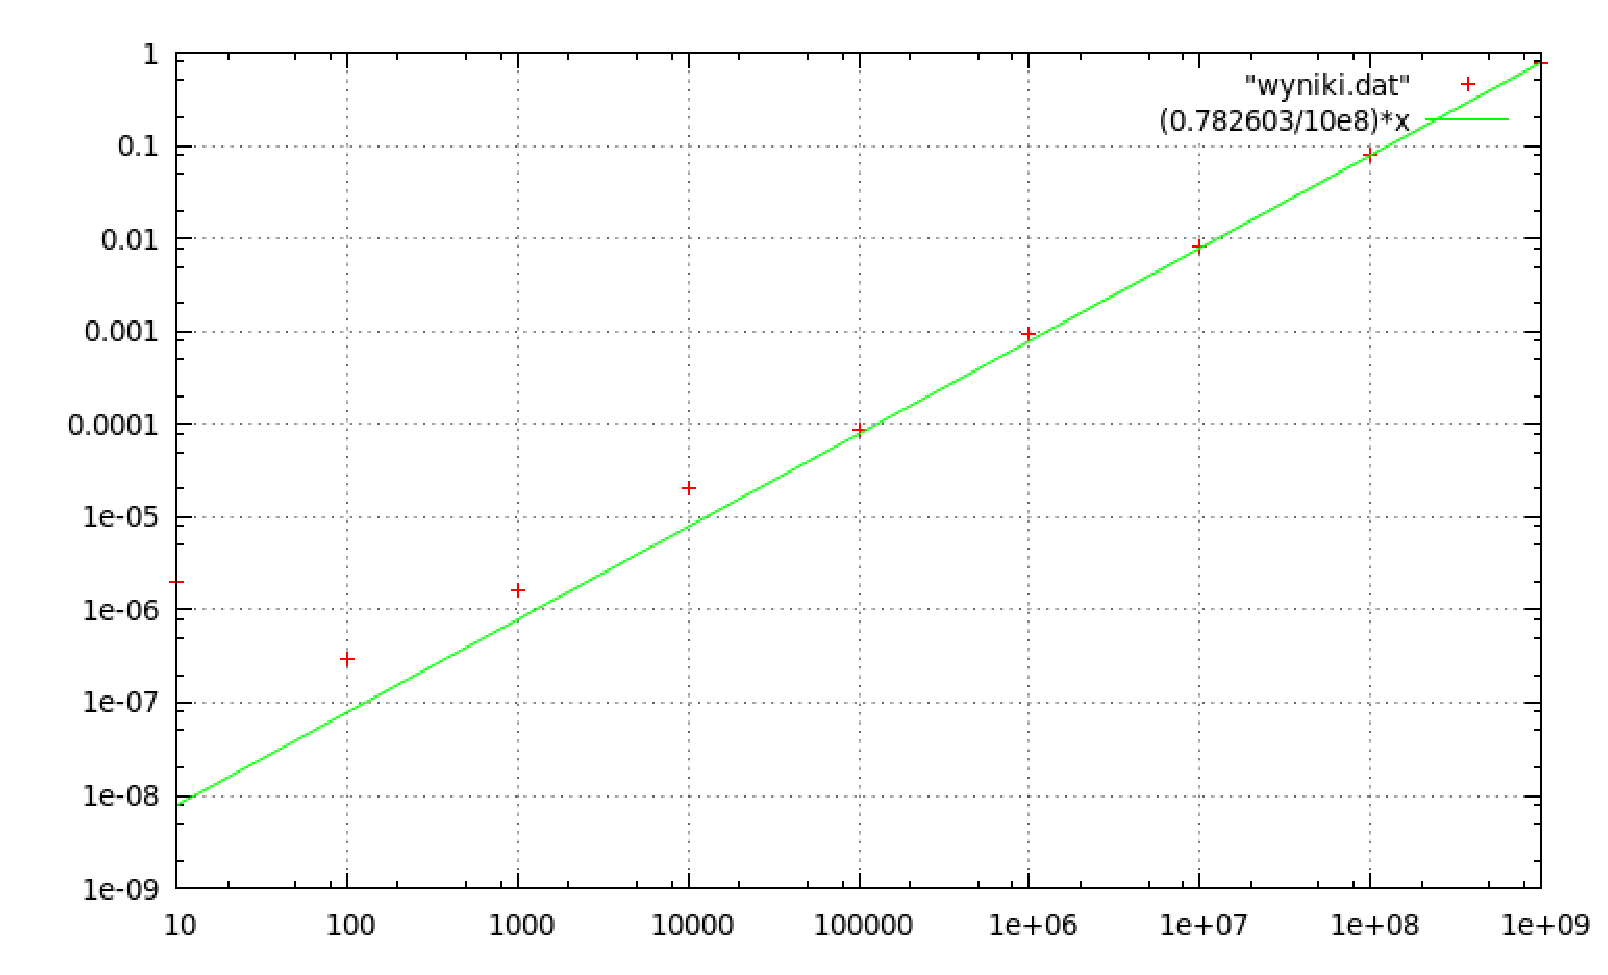
\includegraphics[width=\textwidth,height=\textheight,keepaspectratio]{wykres1.eps}}

\part{Dokumentacja klas}
\hypertarget{structcegla}{\section{Dokumentacja struktury cegla}
\label{structcegla}\index{cegla@{cegla}}
}


Struktura pomocnicza cegla.  




{\ttfamily \#include $<$cegla.\-h$>$}

\subsection*{Metody publiczne}
\begin{DoxyCompactItemize}
\item 
\hyperlink{structcegla_a7a8bf742844b4b9e526454cf49887e78}{cegla} ()
\end{DoxyCompactItemize}
\subsection*{Atrybuty publiczne}
\begin{DoxyCompactItemize}
\item 
int \hyperlink{structcegla_a25ba885f5ac99791f80fd1676ce22a3a}{dana}
\item 
\hyperlink{structcegla}{cegla} $\ast$ \hyperlink{structcegla_aca5144299572d01d919e2655e447f9a8}{nastepna}
\end{DoxyCompactItemize}


\subsection{Opis szczegółowy}
Struktura reprezentuje elementarną cząstkę kontenera -\/ zawiera daną oraz wskaźnik do kolejnego elementu w kontenerze. 

Definicja w linii 15 pliku cegla.\-h.



\subsection{Dokumentacja konstruktora i destruktora}
\hypertarget{structcegla_a7a8bf742844b4b9e526454cf49887e78}{\index{cegla@{cegla}!cegla@{cegla}}
\index{cegla@{cegla}!cegla@{cegla}}
\subsubsection[{cegla}]{\setlength{\rightskip}{0pt plus 5cm}cegla\-::cegla (
\begin{DoxyParamCaption}
{}
\end{DoxyParamCaption}
)\hspace{0.3cm}{\ttfamily [inline]}}}\label{structcegla_a7a8bf742844b4b9e526454cf49887e78}


Definicja w linii 19 pliku cegla.\-h.



\subsection{Dokumentacja atrybutów składowych}
\hypertarget{structcegla_a25ba885f5ac99791f80fd1676ce22a3a}{\index{cegla@{cegla}!dana@{dana}}
\index{dana@{dana}!cegla@{cegla}}
\subsubsection[{dana}]{\setlength{\rightskip}{0pt plus 5cm}int cegla\-::dana}}\label{structcegla_a25ba885f5ac99791f80fd1676ce22a3a}


Definicja w linii 17 pliku cegla.\-h.

\hypertarget{structcegla_aca5144299572d01d919e2655e447f9a8}{\index{cegla@{cegla}!nastepna@{nastepna}}
\index{nastepna@{nastepna}!cegla@{cegla}}
\subsubsection[{nastepna}]{\setlength{\rightskip}{0pt plus 5cm}{\bf cegla}$\ast$ cegla\-::nastepna}}\label{structcegla_aca5144299572d01d919e2655e447f9a8}


Definicja w linii 18 pliku cegla.\-h.



Dokumentacja dla tej struktury została wygenerowana z pliku\-:\begin{DoxyCompactItemize}
\item 
\hyperlink{cegla_8h}{cegla.\-h}\end{DoxyCompactItemize}

\hypertarget{class_kolejka}{\section{Dokumentacja klasy Kolejka}
\label{class_kolejka}\index{Kolejka@{Kolejka}}
}


\hyperlink{class_kolejka}{Kolejka}, abstrakcyjna struktura danych z buforem typu L\-I\-F\-O.  




{\ttfamily \#include $<$kolejka.\-h$>$}

Diagram dziedziczenia dla Kolejka\begin{figure}[H]
\begin{center}
\leavevmode
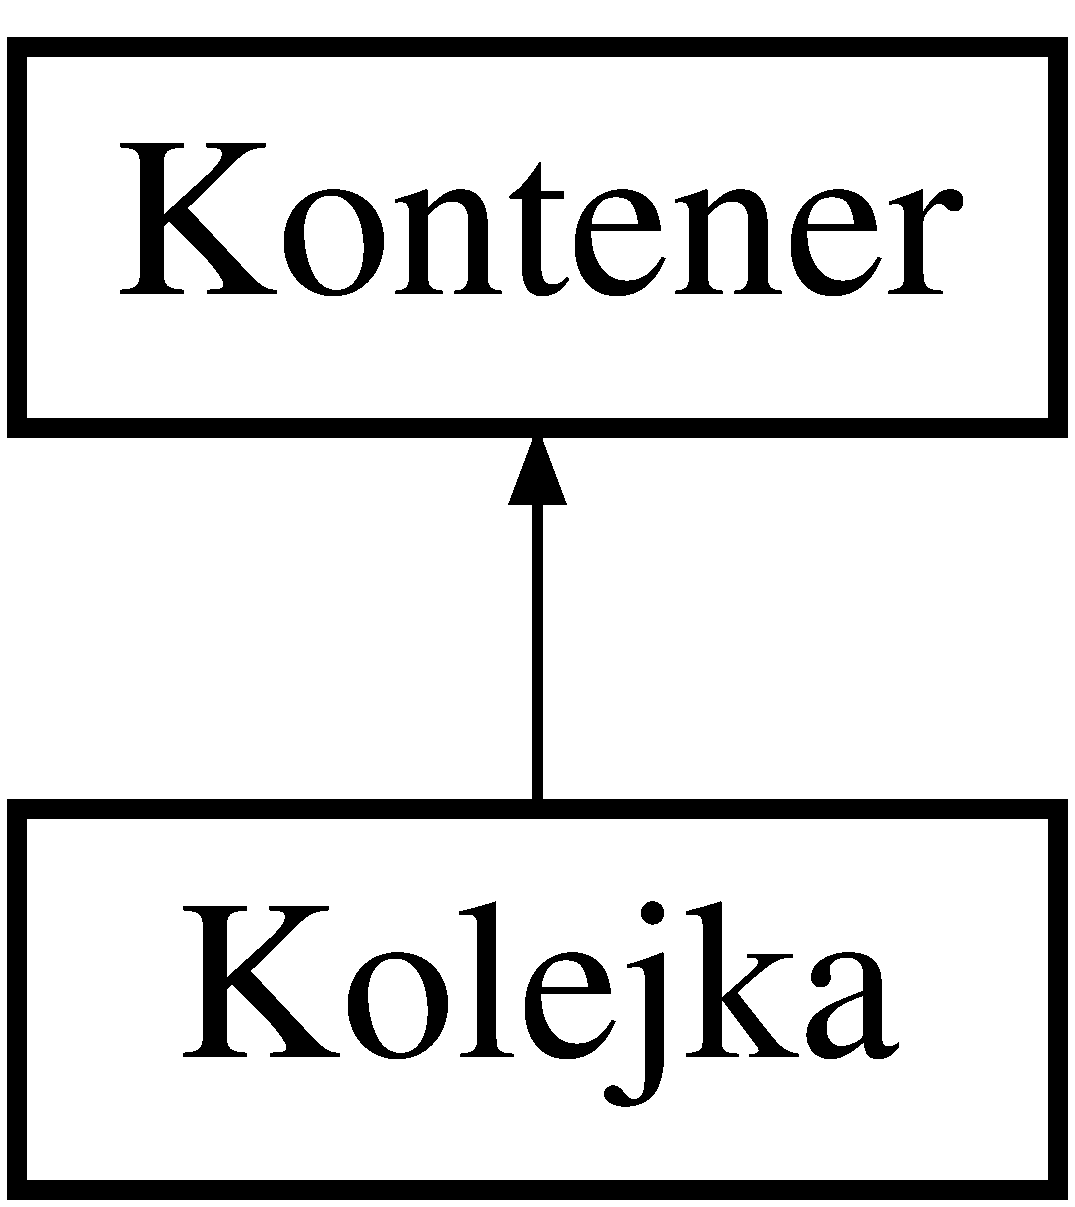
\includegraphics[height=2.000000cm]{class_kolejka}
\end{center}
\end{figure}
\subsection*{Metody publiczne}
\begin{DoxyCompactItemize}
\item 
int \hyperlink{class_kolejka_aa99d7c7459116c2331b301637b45b666}{pop} ()
\begin{DoxyCompactList}\small\item\em Pop kolejki jaki jest, każdy widzi. Usuwa najstarszy element i zwraca wartość przez niego przechowywaną. \end{DoxyCompactList}\end{DoxyCompactItemize}
\subsection*{Dodatkowe Dziedziczone Składowe}


\subsection{Opis szczegółowy}


Definicja w linii 12 pliku kolejka.\-h.



\subsection{Dokumentacja funkcji składowych}
\hypertarget{class_kolejka_aa99d7c7459116c2331b301637b45b666}{\index{Kolejka@{Kolejka}!pop@{pop}}
\index{pop@{pop}!Kolejka@{Kolejka}}
\subsubsection[{pop}]{\setlength{\rightskip}{0pt plus 5cm}int Kolejka\-::pop (
\begin{DoxyParamCaption}
{}
\end{DoxyParamCaption}
)\hspace{0.3cm}{\ttfamily [inline]}}}\label{class_kolejka_aa99d7c7459116c2331b301637b45b666}


Definicja w linii 18 pliku kolejka.\-h.



Dokumentacja dla tej klasy została wygenerowana z pliku\-:\begin{DoxyCompactItemize}
\item 
\hyperlink{kolejka_8h}{kolejka.\-h}\end{DoxyCompactItemize}

\hypertarget{class_kontener}{\section{Dokumentacja klasy Kontener}
\label{class_kontener}\index{Kontener@{Kontener}}
}


{\ttfamily \#include $<$kontener.\-h$>$}

Diagram dziedziczenia dla Kontener\begin{figure}[H]
\begin{center}
\leavevmode
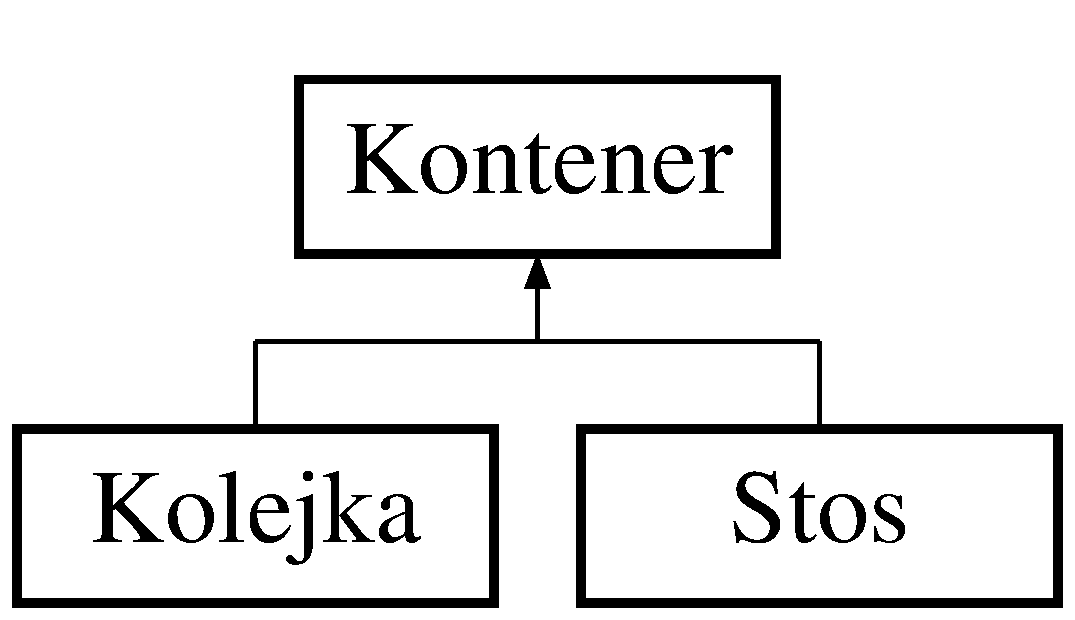
\includegraphics[height=2.000000cm]{class_kontener}
\end{center}
\end{figure}
\subsection*{Metody publiczne}
\begin{DoxyCompactItemize}
\item 
\hyperlink{class_kontener_acfd438daac27e2bce49e3996906fce04}{Kontener} ()
\begin{DoxyCompactList}\small\item\em Konstruktor klasy \hyperlink{class_kontener}{Kontener}. \end{DoxyCompactList}\item 
void \hyperlink{class_kontener_a3809188c7de418862808c5b660df7ff0}{push} (int)
\begin{DoxyCompactList}\small\item\em Wrzuca nową cegiełkę na początek kontenera. \end{DoxyCompactList}\item 
void \hyperlink{class_kontener_a04b49ab497d6a3b0abca2d19089a7981}{insert} (int wartosc, int indeks)
\begin{DoxyCompactList}\small\item\em Umieszcza cegłę z wartością 'wartosc' w miejscu oddalonym o 'indeks' miejsc od początku kontenera. \end{DoxyCompactList}\item 
int \hyperlink{class_kontener_aa1874bdb5728ba2d4d23137733430249}{size} ()
\begin{DoxyCompactList}\small\item\em Liczy z ilu cegiełek składa się kontener. \end{DoxyCompactList}\item 
int \hyperlink{class_kontener_a20830cba10e97685c4dc13253a3cc2ff}{erase} (int)
\begin{DoxyCompactList}\small\item\em Usuwa z listy element o wybranym indeksie. \end{DoxyCompactList}\item 
int \hyperlink{class_kontener_a5b0fd99db2e568ff69fd46131b1bd236}{find} (int)
\begin{DoxyCompactList}\small\item\em Odnajduje w kontenerze przekazaną w argumencie wartość. \end{DoxyCompactList}\item 
void \hyperlink{class_kontener_a1c6af960f6471b9b69a0ec7ebcdc2863}{show} ()
\begin{DoxyCompactList}\small\item\em Wypisuje elementy listy od najmłodszego zaczynając. \end{DoxyCompactList}\end{DoxyCompactItemize}
\subsection*{Atrybuty chronione}
\begin{DoxyCompactItemize}
\item 
\hyperlink{structcegla}{cegla} $\ast$ \hyperlink{class_kontener_aba3ad5cbdc83aa04b18b4237f6a16371}{alfa}
\end{DoxyCompactItemize}


\subsection{Opis szczegółowy}


Definicja w linii 13 pliku kontener.\-h.



\subsection{Dokumentacja konstruktora i destruktora}
\hypertarget{class_kontener_acfd438daac27e2bce49e3996906fce04}{\index{Kontener@{Kontener}!Kontener@{Kontener}}
\index{Kontener@{Kontener}!Kontener@{Kontener}}
\subsubsection[{Kontener}]{\setlength{\rightskip}{0pt plus 5cm}Kontener\-::\-Kontener (
\begin{DoxyParamCaption}
{}
\end{DoxyParamCaption}
)\hspace{0.3cm}{\ttfamily [inline]}}}\label{class_kontener_acfd438daac27e2bce49e3996906fce04}
Konstruktor klasy \hyperlink{class_kontener}{Kontener} inicjalizuje wskaźnik 'alfa' wartością N\-U\-L\-L. 

Definicja w linii 25 pliku kontener.\-h.



\subsection{Dokumentacja funkcji składowych}
\hypertarget{class_kontener_a20830cba10e97685c4dc13253a3cc2ff}{\index{Kontener@{Kontener}!erase@{erase}}
\index{erase@{erase}!Kontener@{Kontener}}
\subsubsection[{erase}]{\setlength{\rightskip}{0pt plus 5cm}int Kontener\-::erase (
\begin{DoxyParamCaption}
\item[{int}]{indeks}
\end{DoxyParamCaption}
)}}\label{class_kontener_a20830cba10e97685c4dc13253a3cc2ff}
Zainicjalizowane są dwa wskaźniki na najmłodszą cegiełkę. Jeden jest ustawiany na element do usunięcia, drugi na element o jeden młodszy. Następuje roszada wskaźników\-: wskaźnik młodszej cegły wskazuje na cegłę starszą od usuwanej, zostaje zapisana wartość przechowywana przez usuwaną cegłę i wreszcie zwolniona zostaje pamięć zajmowana dotychczas przez cegłę. \begin{DoxyReturn}{Zwraca}
Zwraca wartość przechowywaną w usuniętej cegiełce. 
\end{DoxyReturn}


Definicja w linii 58 pliku kontener.\-cpp.

\hypertarget{class_kontener_a5b0fd99db2e568ff69fd46131b1bd236}{\index{Kontener@{Kontener}!find@{find}}
\index{find@{find}!Kontener@{Kontener}}
\subsubsection[{find}]{\setlength{\rightskip}{0pt plus 5cm}int Kontener\-::find (
\begin{DoxyParamCaption}
\item[{int}]{wartosc}
\end{DoxyParamCaption}
)}}\label{class_kontener_a5b0fd99db2e568ff69fd46131b1bd236}
Powołany do życia jest szpieg -\/ wskaźnik na obiekt typu 'cegla', który przemierza kontener w poszukiwaniu najwcześniejszego wystąpienia poszukiwanej wartości. Operacji towarzyszy licznik, który śledzi ilość miniętych przez wskaźnik cegieł, którą metoda zwraca. Należy ją interpretować jako indeks cegły, gdzie najwcześniej wystąpiła poszukiwana wartość.

\begin{DoxyReturn}{Zwraca}
Zwraca indeks (liczony od 0 od najmłodszej cegiełki) najbliższego wystąpienia poszukiwanej wartości. 
\end{DoxyReturn}


Definicja w linii 91 pliku kontener.\-cpp.

\hypertarget{class_kontener_a04b49ab497d6a3b0abca2d19089a7981}{\index{Kontener@{Kontener}!insert@{insert}}
\index{insert@{insert}!Kontener@{Kontener}}
\subsubsection[{insert}]{\setlength{\rightskip}{0pt plus 5cm}void Kontener\-::insert (
\begin{DoxyParamCaption}
\item[{int}]{wartosc, }
\item[{int}]{indeks}
\end{DoxyParamCaption}
)}}\label{class_kontener_a04b49ab497d6a3b0abca2d19089a7981}
U\-W\-A\-G\-A\-: Indeks liczony jest od zera, od najmłodszej cegły. 

Definicja w linii 15 pliku kontener.\-cpp.

\hypertarget{class_kontener_a3809188c7de418862808c5b660df7ff0}{\index{Kontener@{Kontener}!push@{push}}
\index{push@{push}!Kontener@{Kontener}}
\subsubsection[{push}]{\setlength{\rightskip}{0pt plus 5cm}void Kontener\-::push (
\begin{DoxyParamCaption}
\item[{int}]{wart}
\end{DoxyParamCaption}
)}}\label{class_kontener_a3809188c7de418862808c5b660df7ff0}


Definicja w linii 7 pliku kontener.\-cpp.

\hypertarget{class_kontener_a1c6af960f6471b9b69a0ec7ebcdc2863}{\index{Kontener@{Kontener}!show@{show}}
\index{show@{show}!Kontener@{Kontener}}
\subsubsection[{show}]{\setlength{\rightskip}{0pt plus 5cm}void Kontener\-::show (
\begin{DoxyParamCaption}
{}
\end{DoxyParamCaption}
)}}\label{class_kontener_a1c6af960f6471b9b69a0ec7ebcdc2863}


Definicja w linii 108 pliku kontener.\-cpp.

\hypertarget{class_kontener_aa1874bdb5728ba2d4d23137733430249}{\index{Kontener@{Kontener}!size@{size}}
\index{size@{size}!Kontener@{Kontener}}
\subsubsection[{size}]{\setlength{\rightskip}{0pt plus 5cm}int Kontener\-::size (
\begin{DoxyParamCaption}
{}
\end{DoxyParamCaption}
)}}\label{class_kontener_aa1874bdb5728ba2d4d23137733430249}
Zainicjalizowany zostaje wskaźnik na strukturę 'cegla' wskazujący na najmłodszą cegiełkę. Zostaje on potem wysłany w epicką podróż na sam koniec kontenera (czyli do napotkania N\-U\-L\-La). Towarzyszy mu licznik, który zlicza mijane po drodze cegiełki, których ilosć funkcja zwraca.

\begin{DoxyReturn}{Zwraca}
Zwraca wielkość kontenera. 
\end{DoxyReturn}


Definicja w linii 43 pliku kontener.\-cpp.



\subsection{Dokumentacja atrybutów składowych}
\hypertarget{class_kontener_aba3ad5cbdc83aa04b18b4237f6a16371}{\index{Kontener@{Kontener}!alfa@{alfa}}
\index{alfa@{alfa}!Kontener@{Kontener}}
\subsubsection[{alfa}]{\setlength{\rightskip}{0pt plus 5cm}{\bf cegla}$\ast$ Kontener\-::alfa\hspace{0.3cm}{\ttfamily [protected]}}}\label{class_kontener_aba3ad5cbdc83aa04b18b4237f6a16371}


Definicja w linii 16 pliku kontener.\-h.



Dokumentacja dla tej klasy została wygenerowana z plików\-:\begin{DoxyCompactItemize}
\item 
\hyperlink{kontener_8h}{kontener.\-h}\item 
\hyperlink{kontener_8cpp}{kontener.\-cpp}\end{DoxyCompactItemize}

\hypertarget{class_stos}{\section{Dokumentacja klasy Stos}
\label{class_stos}\index{Stos@{Stos}}
}


\hyperlink{class_stos}{Stos}, abstrakcyjna struktura danych z buforem typu F\-I\-F\-O.  




{\ttfamily \#include $<$stos.\-h$>$}

Diagram dziedziczenia dla Stos\begin{figure}[H]
\begin{center}
\leavevmode
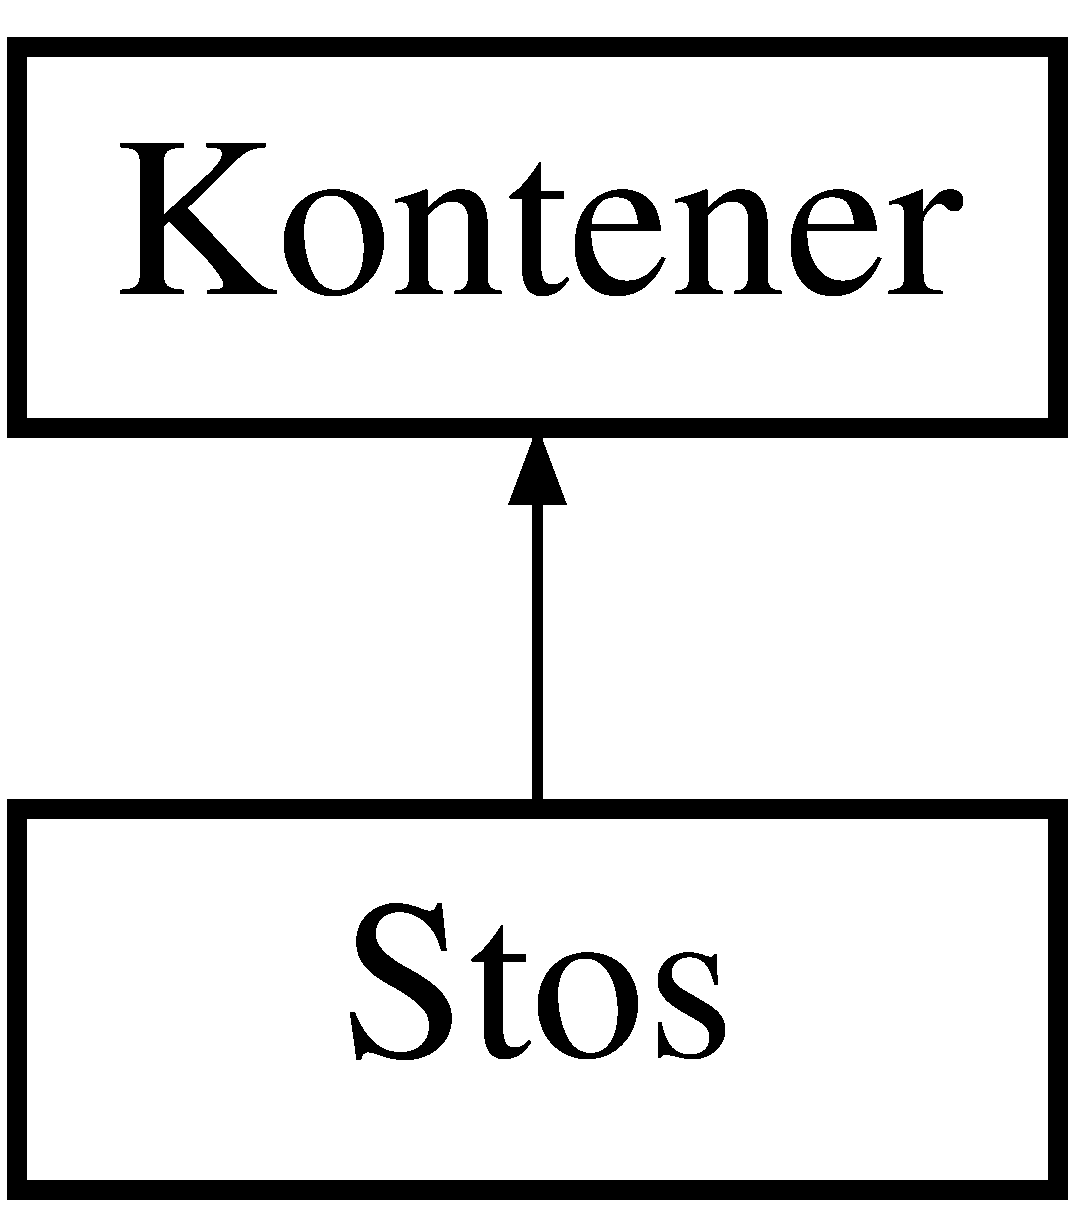
\includegraphics[height=2.000000cm]{class_stos}
\end{center}
\end{figure}
\subsection*{Metody publiczne}
\begin{DoxyCompactItemize}
\item 
int \hyperlink{class_stos_aabb14b8a389c55da6e2b50fbb179ed56}{pop} ()
\begin{DoxyCompactList}\small\item\em Pop stosu jaki jest, każdy widzi. Zdejmuje najmłdoszy element i zwraca wartość przez niego przechowywaną. \end{DoxyCompactList}\end{DoxyCompactItemize}
\subsection*{Dodatkowe Dziedziczone Składowe}


\subsection{Opis szczegółowy}


Definicja w linii 12 pliku stos.\-h.



\subsection{Dokumentacja funkcji składowych}
\hypertarget{class_stos_aabb14b8a389c55da6e2b50fbb179ed56}{\index{Stos@{Stos}!pop@{pop}}
\index{pop@{pop}!Stos@{Stos}}
\subsubsection[{pop}]{\setlength{\rightskip}{0pt plus 5cm}int Stos\-::pop (
\begin{DoxyParamCaption}
{}
\end{DoxyParamCaption}
)\hspace{0.3cm}{\ttfamily [inline]}}}\label{class_stos_aabb14b8a389c55da6e2b50fbb179ed56}


Definicja w linii 18 pliku stos.\-h.



Dokumentacja dla tej klasy została wygenerowana z pliku\-:\begin{DoxyCompactItemize}
\item 
\hyperlink{stos_8h}{stos.\-h}\end{DoxyCompactItemize}

\part{Dokumentacja plików}
\hypertarget{cegla_8h}{\section{Dokumentacja pliku cegla.\-h}
\label{cegla_8h}\index{cegla.\-h@{cegla.\-h}}
}


Plik zawiera definicję struktury pomocniczej cegla.  


\subsection*{Komponenty}
\begin{DoxyCompactItemize}
\item 
struct \hyperlink{structcegla}{cegla}
\begin{DoxyCompactList}\small\item\em Struktura pomocnicza cegla. \end{DoxyCompactList}\end{DoxyCompactItemize}

\hypertarget{kolejka_8h}{\section{Dokumentacja pliku kolejka.\-h}
\label{kolejka_8h}\index{kolejka.\-h@{kolejka.\-h}}
}


Plik zawiera definicję klasy \hyperlink{class_kolejka}{Kolejka} jako pochodnej klasy \hyperlink{class_kontener}{Kontener} oraz definicje jego metod.  


{\ttfamily \#include \char`\"{}kontener.\-h\char`\"{}}\\*
\subsection*{Komponenty}
\begin{DoxyCompactItemize}
\item 
class \hyperlink{class_kolejka}{Kolejka}
\begin{DoxyCompactList}\small\item\em \hyperlink{class_kolejka}{Kolejka}, abstrakcyjna struktura danych z buforem typu L\-I\-F\-O. \end{DoxyCompactList}\end{DoxyCompactItemize}

\hypertarget{kontener_8h}{\section{Dokumentacja pliku kontener.\-h}
\label{kontener_8h}\index{kontener.\-h@{kontener.\-h}}
}


Plik zawiera definicję klasy Kontener oraz deklaracje metod tej klasy.  


{\ttfamily \#include $<$cstdlib$>$}\\*
{\ttfamily \#include $<$iostream$>$}\\*
{\ttfamily \#include \char`\"{}cegla.\-h\char`\"{}}\\*
\subsection*{Komponenty}
\begin{DoxyCompactItemize}
\item 
class \hyperlink{classls_1_1_kontener}{ls\-::\-Kontener}
\end{DoxyCompactItemize}
\subsection*{Przestrzenie nazw}
\begin{DoxyCompactItemize}
\item 
\hyperlink{namespacels}{ls}
\begin{DoxyCompactList}\small\item\em \hyperlink{classls_1_1_kolejka}{Kolejka}, abstrakcyjna struktura danych z buforem typu L\-I\-F\-O. \end{DoxyCompactList}\end{DoxyCompactItemize}

\hypertarget{stos_8h}{\section{Dokumentacja pliku stos.\-h}
\label{stos_8h}\index{stos.\-h@{stos.\-h}}
}


Plik zawiera definicję klasy Stos jako pochodnej klasy Kontener oraz definicje jego metod.  


{\ttfamily \#include \char`\"{}kontener.\-h\char`\"{}}\\*
\subsection*{Komponenty}
\begin{DoxyCompactItemize}
\item 
class \hyperlink{classls_1_1_stos}{ls\-::\-Stos}
\end{DoxyCompactItemize}
\subsection*{Przestrzenie nazw}
\begin{DoxyCompactItemize}
\item 
\hyperlink{namespacels}{ls}
\begin{DoxyCompactList}\small\item\em \hyperlink{classls_1_1_kolejka}{Kolejka}, abstrakcyjna struktura danych z buforem typu L\-I\-F\-O. \end{DoxyCompactList}\end{DoxyCompactItemize}

%--- End generated contents ---

% Index
\newpage
\phantomsection
\addcontentsline{toc}{chapter}{Indeks}
\printindex

\end{document}
